%%
%% This is file `sample-sigconf.tex',
%% generated with the docstrip utility.
%%
%% The original source files were:
%%
%% samples.dtx  (with options: `sigconf')
%% 
%% IMPORTANT NOTICE:
%% 
%% For the copyright see the source file.
%% 
%% Any modified versions of this file must be renamed
%% with new filenames distinct from sample-sigconf.tex.
%% 
%% For distribution of the original source see the terms
%% for copying and modification in the file samples.dtx.
%% 
%% This generated file may be distributed as long as the
%% original source files, as listed above, are part of the
%% same distribution. (The sources need not necessarily be
%% in the same archive or directory.)
%%
%%
%% Commands for TeXCount
%TC:macro \cite [option:text,text]
%TC:macro \citep [option:text,text]
%TC:macro \citet [option:text,text]
%TC:envir table 0 1
%TC:envir table* 0 1
%TC:envir tabular [ignore] word
%TC:envir displaymath 0 word
%TC:envir math 0 word
%TC:envir comment 0 0
%%
%%
%% The first command in your LaTeX source must be the \documentclass
%% command.
%%
%% For submission and review of your manuscript please change the
%% command to \documentclass[manuscript, screen, review]{acmart}.
%%
%% When submitting camera ready or to TAPS, please change the command
%% to \documentclass[sigconf]{acmart} or whichever template is required
%% for your publication.
%%
%%
\documentclass[sigconf]{acmart}

%%
%% \BibTeX command to typeset BibTeX logo in the docs
\AtBeginDocument{%
  \providecommand\BibTeX{{%
    Bib\TeX}}}

%% Rights management information.  This information is sent to you
%% when you complete the rights form.  These commands have SAMPLE
%% values in them; it is your responsibility as an author to replace
%% the commands and values with those provided to you when you
%% complete the rights form.
\setcopyright{acmcopyright}
\copyrightyear{2018}
\acmYear{2018}
\acmDOI{XXXXXXX.XXXXXXX}

%% These commands are for a PROCEEDINGS abstract or paper.
\acmConference[Conference acronym 'XX]{Make sure to enter the correct
  conference title from your rights confirmation emai}{June 03--05,
  2018}{Woodstock, NY}
%%
%%  Uncomment \acmBooktitle if the title of the proceedings is different
%%  from ``Proceedings of ...''!
%%
%%\acmBooktitle{Woodstock '18: ACM Symposium on Neural Gaze Detection,
%%  June 03--05, 2018, Woodstock, NY}
\acmPrice{15.00}
\acmISBN{978-1-4503-XXXX-X/18/06}


%%
%% Submission ID.
%% Use this when submitting an article to a sponsored event. You'll
%% receive a unique submission ID from the organizers
%% of the event, and this ID should be used as the parameter to this command.
%%\acmSubmissionID{123-A56-BU3}

%%
%% For managing citations, it is recommended to use bibliography
%% files in BibTeX format.
%%
%% You can then either use BibTeX with the ACM-Reference-Format style,
%% or BibLaTeX with the acmnumeric or acmauthoryear sytles, that include
%% support for advanced citation of software artefact from the
%% biblatex-software package, also separately available on CTAN.
%%
%% Look at the sample-*-biblatex.tex files for templates showcasing
%% the biblatex styles.
%%

%%
%% The majority of ACM publications use numbered citations and
%% references.  The command \citestyle{authoryear} switches to the
%% "author year" style.
%%
%% If you are preparing content for an event
%% sponsored by ACM SIGGRAPH, you must use the "author year" style of
%% citations and references.
%% Uncommenting
%% the next command will enable that style.
%%\citestyle{acmauthoryear}


%%
%% end of the preamble, start of the body of the document source.
\begin{document}

%%
%% The "title" command has an optional parameter,
%% allowing the author to define a "short title" to be used in page headers.
\title{CS527 midterm report}

%%
%% The "author" command and its associated commands are used to define
%% the authors and their affiliations.
%% Of note is the shared affiliation of the first two authors, and the
%% "authornote" and "authornotemark" commands
%% used to denote shared contribution to the research.
\author{Yiteng Hu}
\authornote{Both authors contributed equally to this research.}
\email{yitengh2@illinois.edu}
\author{Yuehao Shi}
\authornotemark[1]
\email{yuehaos2@illinois.edu}
\affiliation{%
  \institution{UIUC}
  \city{Champaign}
  \state{IL}
  \country{USA}
  \postcode{61801}
}

%%
%% By default, the full list of authors will be used in the page
%% headers. Often, this list is too long, and will overlap
%% other information printed in the page headers. This command allows
%% the author to define a more concise list
%% of authors' names for this purpose.
\renewcommand{\shortauthors}{Trovato et al.}

%%
%% The abstract is a short summary of the work to be presented in the
%% article.
\begin{abstract}
  The article presents an extension of the FreeFuzz automated fuzz testing tool to test PaddlePaddle, 
  an emerging open-source deep learning library. The team aims to improve the reliability of deep learning 
  libraries by identifying and fixing potential bugs and vulnerabilities. The proposed solution involves 
  four steps: code collection, instrumentation, mutation test, and oracle test. The team has completed 
  the code collection and instrumentation stages, while the mutation stage is yet to be completed. 
  The team has encountered challenges due to different installation settings and environments for
   TensorFlow and PaddlePaddle packages and insufficient data collection, delaying the mutation strategy development.
    The team plans to use metrics such as covered APIs, the size of the value space, and line coverage to evaluate the effectiveness 
    of the Freefuzz tests for PaddlePaddle and compare them to other state-of-the-art deep learning library testing techniques.
\end{abstract}

%%
%% The code below is generated by the tool at http://dl.acm.org/ccs.cfm.
%% Please copy and paste the code instead of the example below.
%%

%%
%% Keywords. The author(s) should pick words that accurately describe
%% the work being presented. Separate the keywords with commas.
\keywords{Fuzz testing, Deep learning libraries, PaddlePaddle, Automated testing, Mutation testing}
%% A "teaser" image appears between the author and affiliation
%% information and the body of the document, and typically spans the
%% page.


%%
%% This command processes the author and affiliation and title
%% information and builds the first part of the formatted document.
\maketitle

\section{problem statement}
Freefuzz is an automated fuzz testing tool that has been developed for deep learning 
libraries like Pytorch and Tensorflow. This powerful tool helps developers identify potential 
issues that may be overlooked during manual testing. However, Freefuzz has not developed tests for
 PaddlePaddle, which is an emerging open-source deep learning library. To address this challenge, 
 the project team aims to extend the existing fuzzing system to test PaddlePaddle. The goal is to 
 improve the reliability of these libraries by discovering and fixing potential bugs and vulnerabilities.

\section{Background}
Deep learning libraries play a crucial role in our daily lives, but bugs in these systems can have disastrous 
consequences.Surprisingly, despite the importance of DL library reliability, there is only limited work for testing
 DL libraries. One example of this is CRADLE, which uses pre-existing DL models to test Keras and its backends, 
 and addresses the issue of test oracles through differential testing. To expand on this approach, LEMON enhances 
 CRADLE by utilizing various model mutation rules to create a wider range of DL models. This enables the invocation 
 of more library code and exposes a greater number of potential bugs in the DL library.
\section{Proposed solution}
The team will use the FreeFuzz approach to test PaddlePaddle library, which involves four steps: code collection, 
instrumentation, mutation test, and oracle test. In code collection, we will gather documentation code, library tests,
 and deep learning models. Next, we will perform type inference and identify input and output data types in instrumentation.
  Then, we will carry out type, random value, and database value mutation tests. Finally, we will perform differential tests 
  and metamorphic testing in the oracle test. This approach can help efficiently and effectively test the library.
  \begin{figure}[h]
    \centering
    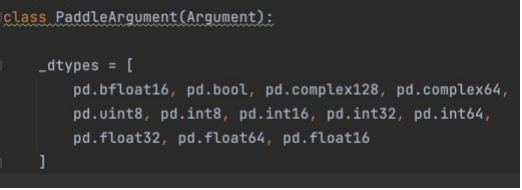
\includegraphics[width=\linewidth]{4.png}
    \caption{Four steps of Freefuzz}
  \end{figure}  
\section{Evaluation}
The team will use a set of metrics to evaluate the effectiveness of Freefuzz tests for PaddlePaddle. 
These metrics include the number of covered APIs, the size of the value space, and line coverage. 
Additionally, we will compare the Freefuzz testing metrics with those of other state-of-the-art deep learning library testing techniques,
 such as LEMON and CRADLE. By assessing these metrics, the team hopes to determine the strengths and weaknesses of Freefuzz testing and how it compares to other approaches.
  This information will help us to improve their testing process and ensure the quality of PaddlePaddle.
 At present, the team has not amassed a sufficient quantity of API and value space data, precluding the provision of evaluation results up to this point. In light of this, 
the team is currently engaged in an exploration of the potential application of Lemon and Cradle in order to facilitate a comparison of the results of the final fuzzing tests.
\par Currently, the team has not collected enough API and value space data, which prevents them from providing evaluation results.
 Therefore, the team is currently investigating the use of testing tools such as Lemon and Cradle, which have adapted the PaddlePaddle library 
 to compare the results of final fuzzing tests. In the next stage, the team plans to include the total number of bugs found in the evaluation results.

\section{Initial results}
\subsection{Code Collection}
Following the methodology outlined in the paper, implementing FreeFuzz for PaddlePaddle involves four stages. 
The team has completed a portion of Stage 1 and has verified the feasibility of proceeding with later stages. 
Stage 1, referred to as code collection, involves acquiring relevant data sources such as library documentations,
 library developer tests, and open-source packages to support subsequent instrumentation and mutation tasks. 
 The team has collected several PaddlePaddle APIs from the official documentation for the purpose of instrumentation and mutation.
  The team is writing python scraping scripts for API definitions and execution information using bs4 package. For example, 
  five APIs are included in Figure 1 and have been collected during the instrumentation phase.
  \par The team attempted to obtain API execution data from PaddlePaddle test documentation by running the testing 
  files directly on their local machine. Unfortunately, the test files required additional datasets and requirements, 
  causing the PaddlePaddle package to crash during execution. As a result, the team made the decision to temporarily halt 
  the collection of API execution data from test documentations in order to focus on ensuring that the subsequent stages of the project were functioning correctly.
   In the next phase of the project, the team plans to devise a more effective approach to avoid encountering tests with unexpected requirements.

  \begin{figure}[h]
    \centering
    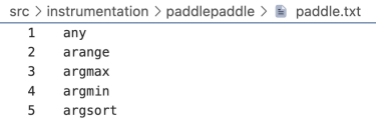
\includegraphics[width=\linewidth]{1.png}
    \caption{Sample APIs collected in Stage 1}
  \end{figure}  
\subsection{instrumentation}
The Freefuzz adaptation process for PaddlePaddle consists of two stages. The second stage involves dynamic tracing with instrumentation, where Freefuzz intercepts selected PaddlePaddle APIs and appends hijacking functions into package installation paths. These hijacking functions execute the collected code from the official documentation, enabling Freefuzz to trace the value and type of all parameters used to execute an API. The collected data is then stored in MongoDB in JSON format to create the necessary type space, API value space, and argument value space for later fuzzing stages.
To implement this instrumentation stage, the team repurposed the code used for testing the PyTorch library, 
utilizing functions such as hijack, decorate-class, decorate-function, and write-fn.
 Currently, the team has only collected APIs from the paddle package to test the feasibility of instrumentation for PaddlePaddle. 
 However, the team was successful in adding the API value space and argument value space to MongoDB for future development after 
 adding the instrumentation code and executing the corresponding API from the official documentation. 
 The API value space collected is displayed in Figure 2.
 \begin{figure}[h]
  \centering
  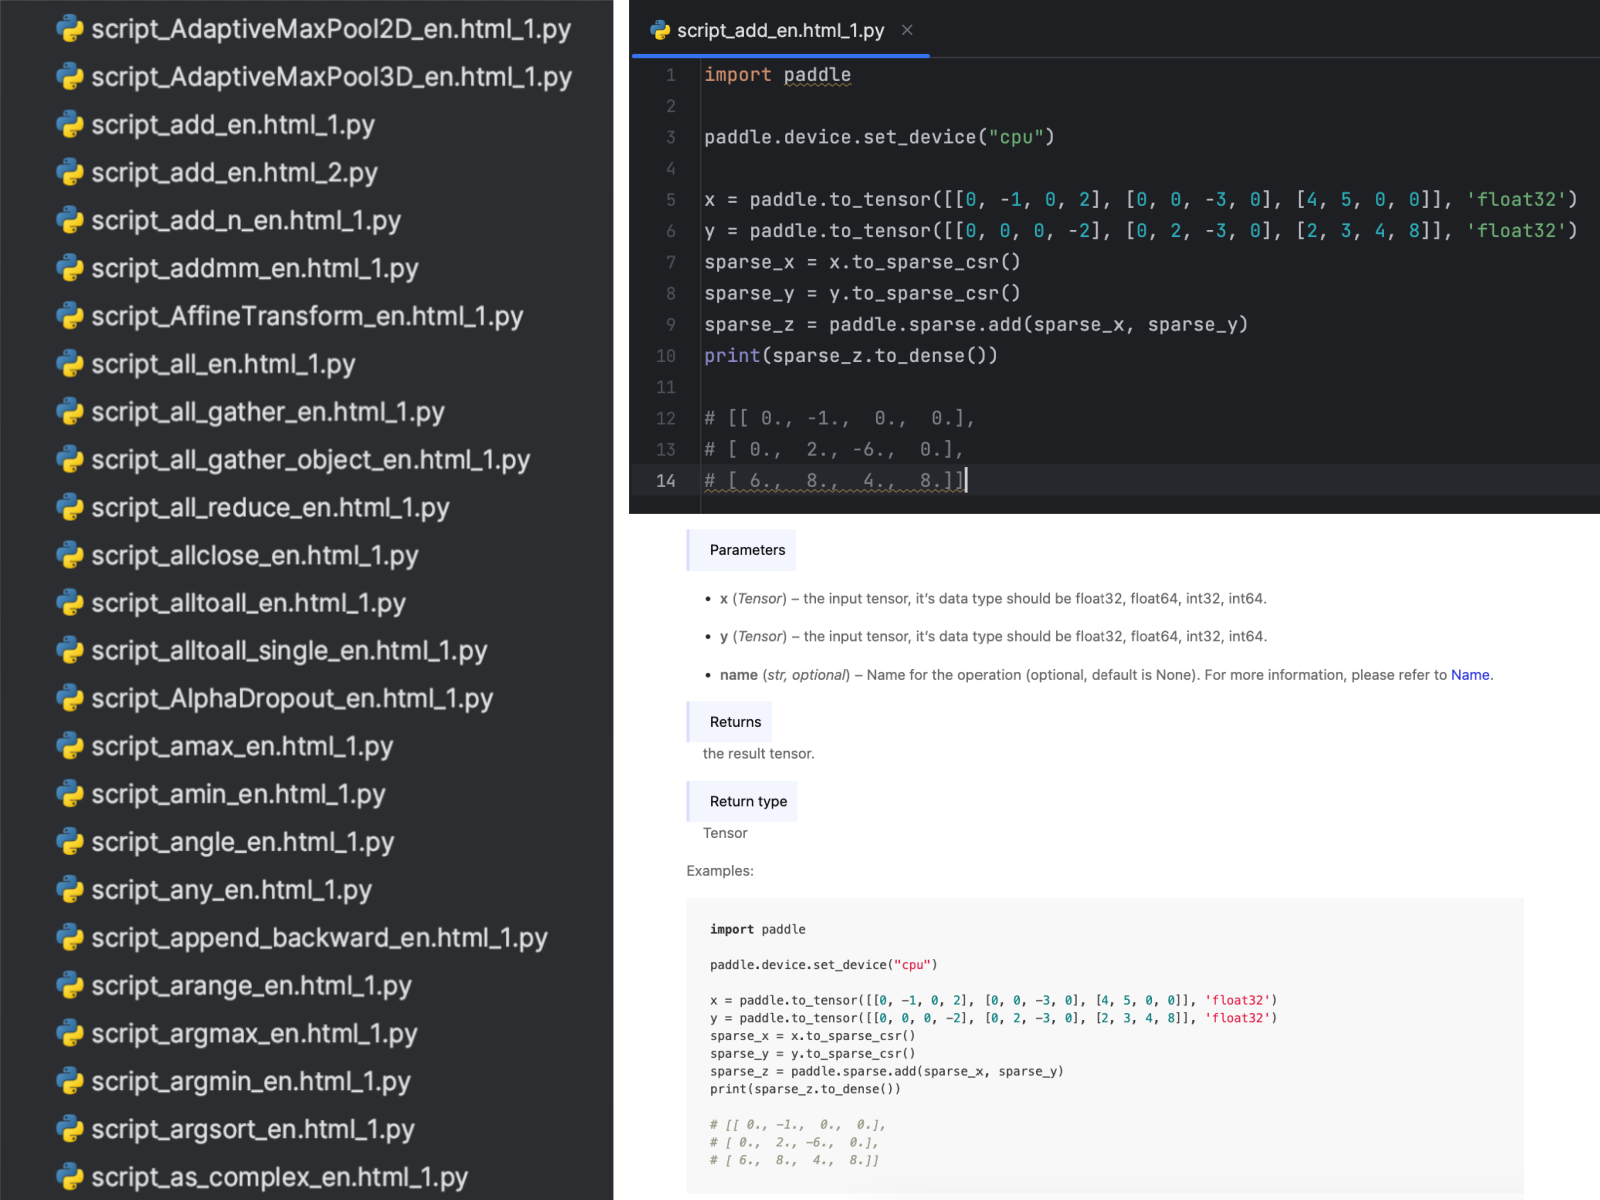
\includegraphics[width=\linewidth]{2.png}
  \caption{Sample API value space collected in MongoDB}
\end{figure}

\subsection{Mutation Test}
We collected different types for PaddlePaddle, which are shown in the figure3. 
And we decide to extend the mutation strategies used in the original paper.
To summarize, the team has selected a subset of APIs as a proof of concept to 
demonstrate the feasibility of applying the complete Freefuzz testing process to the PaddlePaddle package, 
as set out in the midterm goals.
\begin{figure}[h]
  \centering
  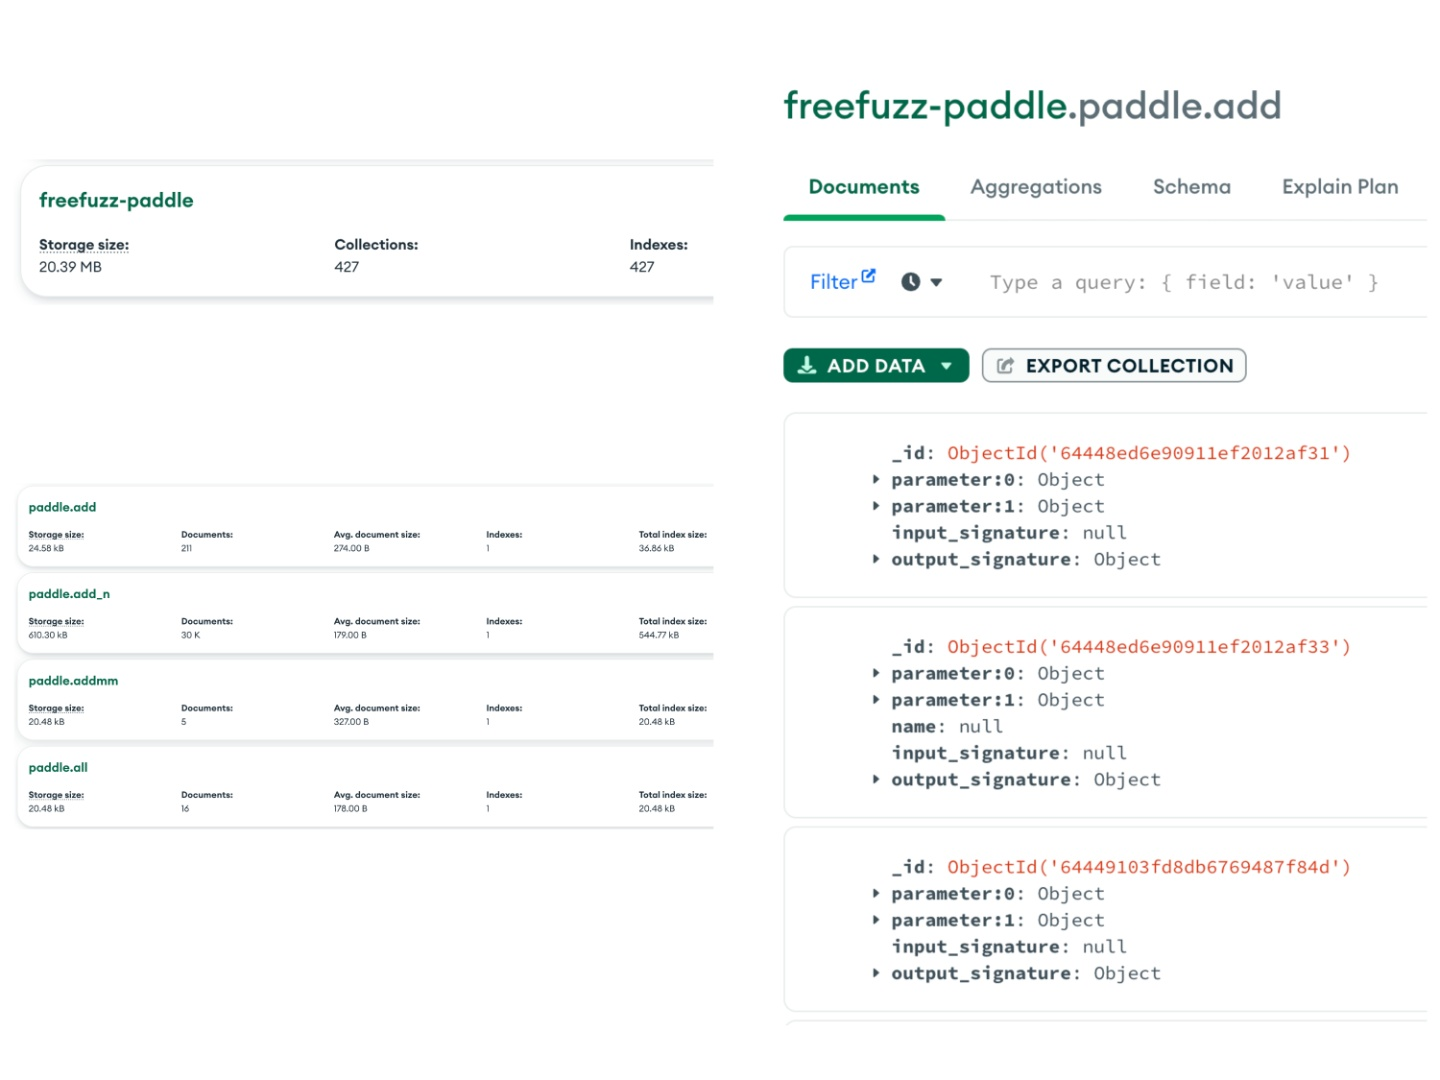
\includegraphics[width=\linewidth]{3.png}
  \caption{data types in PaddlePaddle}
\end{figure}

\section{Challenges and Future Plan}
In general, the team has made good progress towards achieving the midterm goals except for the mutation strategy script in stage 3. However, the team encountered some challenges that slowed down the development process. One of the team members was using a MacOS device with an M1 chip, which required different installation settings and environments for TensorFlow and PaddlePaddle packages compared to general MacOS installation instructions. This unexpected issue took some time for the team to resolve. Additionally, developing a mutation strategy was challenging without sufficient data collection from stage 1. As a result, the team has decided to postpone the development of this part until stage 1 is almost complete.
\par As previously mentioned, the team used a limited number of PaddlePaddle APIs in the midterm to initiate the project. To increase the sample size, the team is currently developing Python crawler scripts to collect additional APIs from official documentation, test documents, and open source projects.
\par The third stage of Freefuzz involves mutation-based fuzzing, where FreeFuzz will generate mutants for the test inputs collected from stage 2. At this point, the team has not developed a mutation strategy but plans to implement type mutation, random value mutation, and database value mutation in the next phase of work. The fourth stage entails running all the generated tests with oracles. Currently, with the collected unmutated API values, there have been no crash or runtime error outputs, which is as expected. In the next phase, the team plans to run the mutated code and generate more oracles to try to find bugs in the PaddlePaddle packages.
\par Finally, the team will evaluate the effectiveness of the Freefuzz testing methodology by measuring the number of covered APIs, the size of the value space, and line coverage. Additionally, they will compare the Freefuzz testing metrics with those of LEMON and CRADLE.
With the successful setup of the development environment and a deeper understanding of Freefuzz, the team is confident that they can complete one functionality in each paragraph mentioned above each week before the final deadline and complete the project on time.

\section{github link}
https://github.com/yuehaoshi/FreeFuzz
\begin{thebibliography}{9}
\bibitem{w1} Wei, A., Deng, Y., Yang, C.,  Zhang, L. (2022, May). Free lunch for testing: Fuzzing deep-learning libraries from open source. In Proceedings of the 44th International Conference on Software Engineering (pp. 995-1007).
\end{thebibliography}
\end{document} 
\endinput
%%
%% End of file `sample-sigconf.tex'.
